%%%%%%%%%%%%%%%%%%%%%%%%%%%%%%%%%%%%%%%%%%%%%%%%%%%%%%%%%%%%%%%%%%%%%%%%%%%%%%%%
% ISE Lab -- Topic
% Giovanni Ciatto
% Alma Mater Studiorum - Università di Bologna
% mailto:giovanni.ciatto@unibo.it
%%%%%%%%%%%%%%%%%%%%%%%%%%%%%%%%%%%%%%%%%%%%%%%%%%%%%%%%%%%%%%%%%%%%%%%%%%%%%%%%
%\documentclass[handout]{beamer}\mode<handout>{\usetheme{default}}
%
\documentclass[presentation]{beamer}\mode<presentation>{\usetheme{AMSBolognaFC}}
%\documentclass[handout]{beamer}\mode<handout>{\usetheme{AMSBolognaFC}}
%%%%%%%%%%%%%%%%%%%%%%%%%%%%%%%%%%%%%%%%%%%%%%%%%%%%%%%%%%%%%%%%%%%%%%%%%%%%%%%%
\usepackage{ise-lab-common}
\usepackage{ise-lab-inference}
% version
\newcommand{\versionmajor}{1}
\newcommand{\versionminor}{0}
\newcommand{\versionpatch}{0-dev}
\newcommand{\version}{\versionmajor.\versionminor.\versionpatch}
%%%%%%%%%%%%%%%%%%%%%%%%%%%%%%%%%%%%%%%%%%%%%%%%%%%%%%%%%%%%%%%%%%%%%%%%%%%%%%%%
\title[\currentLab{} -- Inference]{Automatic Inference on Horn Clauses}
%
\subtitle{\courseName{} / Module \moduleN{} (\courseAcronym)}
%
\author[\sspeaker{\gcShort}]{\speaker{\gcFull} \\ \gcEmail}
%
\institute[\disiShort, \uniboShort]{\disi{} (\disiShort)\\\unibo}
%
\date[A.Y. \academicYear{} (v.\ \version)]{Academic Year \academicYear{}\\(version \version)}
%
%%%%%%%%%%%%%%%%%%%%%%%%%%%%%%%%%%%%%%%%%%%%%%%%%%%%%%%%%%%%%%%%%%%%%%%%%%%%%%%%
\begin{document}
%%%%%%%%%%%%%%%%%%%%%%%%%%%%%%%%%%%%%%%%%%%%%%%%%%%%%%%%%%%%%%%%%%%%%%%%%%%%%%%%

%/////////
\frame{\titlepage}
%/////////

%%===============================================================================
\section*{Outline}
%%===============================================================================
%
%%/////////
\frame[c]{\tableofcontents[hideallsubsections]}
%%/////////

%===============================================================================
\section{Premises}
%===============================================================================

\begin{frame}{Lecture Goals}
    \begin{itemize}
        \item Understand basic notions concerning the \alert{manipulation} of Horn clauses
        %
        \begin{itemize}
            \item substitutions
            \item unification and (most general) unifiers
        \end{itemize}

        \vfill

        \item Understand how these notions can be exploited for \alert{automated inference}
        %
        \begin{itemize}
            \item using the SL\ccite{Robinson1965} resolution principle\ldots
            \item \ldots as suggested by \cite{KowVan1970} (SLD)
        \end{itemize}

        \vfill

        \item Understand the notion of \alert{proof tree}
        %
        \begin{itemize}
            \item and the different possible strategies for its \alert{exploration}
        \end{itemize}
    \end{itemize}
\end{frame}

%===============================================================================
\section{Substitutions and their Application to Logic Formul\ae{}}
%===============================================================================

\begin{frame}{Overview}
    \begin{itemize}
        \item[$\checkmark$] Three main ingredients:
        %
        \begin{description}\small
            \item[terms] --- for representing entities
            \item[predicates] --- for representing statements about entities
            \item[clauses] --- for representing properties of entities or relations among them
        \end{description}

        \vfill

        \item[$\checkmark$] Many ways of representing knowledge through them:
        %
        \begin{description}\small
            \item[extensional vs. intensional] $\approx$ explicitly vs. implicitly
            \item[propositional vs. relational] $\approx$ in tabular form vs. as a graph
        \end{description}

        \vfill

        \item One powerful tool:
        %
        \begin{description}\small
            \item[resolution] --- allowing for \alert{intensional} representations, programming, reasoning, \ldots
        \end{description}

        \vfill

        \item[$\rightarrow$] Two fundamental mechanisms for manipulating knowledge:
        %
        \begin{description}\small
            \item[substitution application] $\approx$ rewriting a formula by assigning variables
            \item[most general unifier] $\approx$ computing the substitution making 2 formul\ae{} equal
        \end{description}
    \end{itemize}
\end{frame}

\subsection{Substitutions}

\begin{frame}[allowframebreaks]{Substitutions}
    \begin{block}{Purpose}\centering
        Denoting variables assignemnts
    \end{block}
    %
    \begin{block}{Informal definition}
        A (possibly \emph{empty}) set of \alert{variable--term} pairs
    \end{block}
    %
    \begin{alertblock}{Formal syntax\hfill\textbf{\footnotesize(same syntactic notation as in \cite{lectures:ise-kr})}}
        \begin{center}
            $\begin{array}{rcl}
                \meta{Substitution} & := & \terminal{\varnothing} \mid \terminal{\{} \meta{Assignemnts} \terminal{\}}
                \\
                \meta{Assignments} & := & \meta{Assignment} \mid \meta{Assignments} \terminal{,} \meta{Assignments}
                \\
                \meta{Assignment} & := & \meta{Variable} \terminal{\mapsto} \meta{Term}
                \\
                \meta{Term} & := & \text{see lecture \cite{lectures:ise-kr}}
				\\
                \meta{Variable} & := & \text{see lecture \cite{lectures:ise-kr}}
			\end{array}$
        \end{center}
    \end{alertblock}

    \begin{exampleblock}{Examples}
        \begin{description}
            \item[$\varnothing$] --- the empty substitution (no variable to be assigned)
            \item[$\{ \variable{X} \mapsto \functor{a} \}$] --- the substitution assigning variable $\variable{X}$ with the constant $\functor{a}$
            \item[$\{ \variable{X} \mapsto \functor{a}, \variable{Y} \mapsto \functor{b} \}$] --- the substitution assigning 
            %
			\begin{itemize}
				\item variable $\variable{X}$ with the constant $\functor{a}$, and
				\item variable $\variable{Y}$ with the constant $\functor{b}$ 
			\end{itemize} 
        \end{description}
    \end{exampleblock}
\end{frame}

\subsection{Substitution Application}

\begin{frame}[allowframebreaks]{Applying Substitutions to Logic Formul\ae{}}
    \begin{block}{Purpose}\centering
        Actually assigning some formula's variables with some values, as denoted by some given substitution
    \end{block}
    %
    \begin{block}{Informal definition}
        The operation by which 
		%
		\begin{enumerate}
			\item a formula (i.e. a term, a predicate, or a Horn cluase) \ldots
			\item \ldots is \alert{rewritten} \ldots
			\item \ldots by \alert{replacing} all variables therein contained \ldots
			\item \ldots with some other \alert{terms}, as prescribed by a given \alert{substitution}
		\end{enumerate}
    \end{block}
	%
    \begin{block}{Notation}
        \begin{itemize}
			\item We denote by 
			%
			\[ \Phi / \sigma \qquad \equiv \Phi'\]
			%
			the operation of applying a substitution $\sigma$ to some formula $\Phi$
			%
			\begin{itemize}
				\item hence producing a new formula $\Phi$
			\end{itemize}

			\item Notice that:
			%
			\begin{itemize}
				\item $(\cdot / \cdot)$ is a function mapping formul\ae{} and substitutions to other formul\ae{}
				\item we denote substitutions by lowercase greek letters such as $\sigma$, $\rho$, etc.
				\item we denote formul\ae{} by uppercase greek letters such as $\Phi$, $\Psi$, etc.
			\end{itemize} 
		\end{itemize}
    \end{block}
    %
    \begin{alertblock}{Formal definition}
		Let $\Phi, \Psi, \Psi', \Psi_1, \ldots, \Psi_n$ be logic formul\ae{} (i.e. terms, predicates, or a Horn cluases) of any sort, 
		%
		let $\predication{p}$ be a $n$-ary predication, let $\functor{f}$ be a $m$-ary functor, let $\functor{k}$ be a constant, let $t$ be a term of any sort,
		%
		and let $\sigma$ be a (possibly empty) substitution;
		%
		then
		
		$$\Phi / \sigma = \begin{cases}
			\Psi / \sigma \Leftarrow \Psi' / \sigma & \text{if} ~ \Phi \equiv \Psi \Leftarrow \Psi'
			\\
			\Psi / \sigma \wedge \Psi' / \sigma & \text{if} ~ \Phi \equiv \Psi \wedge \Psi'
			\\
			\predication{p}(\Psi_1 / \sigma, \ldots, \Psi_n / \sigma) & \text{if} ~ \Phi \equiv \predication{p}(\psi_1, \ldots, \psi_n)
			\\
			\functor{f}(\Psi_1 / \sigma, \ldots, \Psi_m / \sigma) & \text{if} ~ \Phi \equiv \functor{f}(\psi_1, \ldots, \psi_m)
			\\
			\functor{k} & \text{if} ~ \Phi \equiv \functor{k}
			\\
			t & \text{if} ~ \Phi \equiv \variable{X} ~ \text{and} ~ (\variable{X} \mapsto t) \in \sigma
			\\
			\variable{X} & \text{if} ~ \Phi \equiv \variable{X} ~ \text{and} ~ (\variable{X} \mapsto t) \not\in \sigma
		\end{cases}$$
    \end{alertblock}

    \begin{exampleblock}{Examples}
        \begin{itemize}
            \item[] \alert{$\functor{f}(\variable{X}) \ /\  \varnothing$} $\equiv$ $\functor{f}(\variable{X})$
            %
			\begin{itemize}
				\item applying empty substitutions to formul\ae{} has no effect
			\end{itemize} 

			\item[] \alert{$\functor{k} \ /\  \sigma$} $\equiv$ $\functor{k}$
            %
			\begin{itemize}
				\item applying substitutions to constants has no effect
			\end{itemize} 

			\item[] \alert{$\predication{p}(X, \functor{f}(Y)) \ /\  \{ X \mapsto \functor{a}, Y \mapsto \functor{b} \}$} $\equiv$ $\predication{p}(\functor{a}, \functor{f}(\functor{b}))$
            %
			\begin{itemize}
				\item applying substitutions to formul\ae{} replaces the variables therein contained\ldots
			\end{itemize} 

			\item[] \alert{$\predication{p}(X, \functor{f}(Y)) \ /\  \{ X \mapsto \functor{a} \}$} $\equiv$ $\predication{p}(\functor{a}, \functor{f}(Y))$
            %
			\begin{itemize}
				\item \ldots provided that the variable is contained in the substitution\ldots
			\end{itemize} 

			\item[] \alert{$\predication{p}(X, \functor{f}(Y)) \ /\  \{ X \mapsto \functor{a}, Z \mapsto \functor{b} \}$} $\equiv$ $\predication{p}(\functor{a}, \functor{f}(Y))$
            %
			\begin{itemize}
				\item \ldots and in the formula
			\end{itemize} 
        \end{itemize}
    \end{exampleblock}
\end{frame}

\subsection{Refreshing Formul\ae{}}

\begin{frame}[allowframebreaks]{Refreshing Formul\ae{}}
    \begin{block}{Purpose}
        Allowing a formula to be re-used in different contexts, avoiding undesired variable assignments 
		%
		\begin{itemize}
			\item this is not relevant in theory, but very important in practice
		\end{itemize}
    \end{block}
    %
    \begin{block}{Informal definition}
        A formula is \alert{refreshed} by 
		%
		\begin{itemize}
			\item \emph{consistently} replacing each variable therein contained
			\item with some \emph{bare new}\footnote{never used before} variable of similar name 
		\end{itemize}
    \end{block}
    %
    \begin{alertblock}{Formal definition}
		Let 
		%
		\begin{itemize}
			\item \alert{$\Phi$} be a formula (i.e. term, predicate, or Horn cluase) of any sort 
			\item \alert{$\rho = \{ \variable{X} \mapsto \hat{\variable{X}} \mid \forall \variable{X} \in \Phi \}$} be the refreshing substitution for $\Phi$
			%
			\begin{itemize}\small
				\item where $\hat{\variable{X}}$ is a variable which has \alert{never been used before}
			\end{itemize} 
		\end{itemize}
		%
		then we define ``refreshing $\Phi$'' as the operation of applying $\rho$ to $\Phi$:hat
		%
		\begin{center}
			$ \text{refresh}(\Phi) = \alert{\Phi / \rho} $
		\end{center}
    \end{alertblock}

    \begin{exampleblock}{Examples}
        \begin{multicols}{2}\small
			\begin{itemize}
				\item $\text{refresh}(\alert{\functor{f}(\variable{X}, \functor{g}(\variable{X}))})$ 
				\item $\text{refresh}(\alert{\predication{p}(\variable{X}, \functor{f}(\variable{Y}), \functor{g}(\variable{X}))})$ 
				\item $\text{refresh}(\alert{\predication{list}([\variable{H} \mid \variable{T} ])) \Leftarrow \predication{list}(\variable{T})})$ 
				
				\item[$=$] $\functor{f}(\hat{\variable{X}}, \functor{g}(\hat{\variable{X}}))$
				\item[$=$] $\predication{p}(\hat{\variable{X}}, \functor{f}(\hat{\variable{Y}}), \functor{g}(\hat{\variable{X}}))$
				\item[$=$] $\predication{list}([\hat{\variable{H}} \mid \hat{\variable{T} ]})) \Leftarrow \predication{list}(\hat{\variable{T}})$
			\end{itemize}
		\end{multicols}
    \end{exampleblock}
\end{frame}

%===============================================================================
\section{Unification}
%===============================================================================

\begin{frame}{Overview}
    \begin{itemize}
        \item[$\checkmark$] Three main ingredients:
        %
        \begin{description}\small
            \item[terms] --- for representing entities
            \item[predicates] --- for representing statements about entities
            \item[clauses] --- for representing properties of entities or relations among them
        \end{description}

        \vfill

        \item[$\checkmark$] Many ways of representing knowledge through them:
        %
        \begin{description}\small
            \item[extensional vs. intensional] $\approx$ explicitly vs. implicitly
            \item[propositional vs. relational] $\approx$ in tabular form vs. as a graph
        \end{description}

        \vfill

        \item One powerful tool:
        %
        \begin{description}\small
            \item[resolution] --- allowing for \alert{intensional} representations, programming, reasoning, \ldots
        \end{description}

        \vfill

        \item[$\rightarrow$] Two fundamental mechanisms for manipulating knowledge:
        %
        \begin{description}\small
            \item[substitution application] $\approx$ rewriting a formula by assigning variables
            \item[most general unifier] $\approx$ computing the substitution making 2 formul\ae{} equal
        \end{description}
    \end{itemize}
\end{frame}

\begin{frame}[allowframebreaks]{Unification}
    \begin{block}{Purpose}
        Compute which variables assignment may let a given formula
        %
        \begin{itemize}
            \item be equal to another one
            \item hence fitting a particular context
        \end{itemize}
    \end{block}
    %
    \begin{block}{Informal definition}
        The operation by which one may compute
        %
        \begin{itemize}
            \item an \alert{unifier} among any two formul\ae{}
            %
            \begin{itemize}
                \item[ie] a \alert{substitution} making the two formul\ae{} \alert{syntactically equal}
            \end{itemize}

            \item or figure out that it is impossible to do so
        \end{itemize}
    \end{block}
    %
    \begin{alertblock}{Formal definition}
        \begin{center}
            $\text{unify}(\Phi, \Psi) = \begin{cases}
                \sigma & \text{if} ~ \exists \sigma : \Phi = \Psi / \sigma
                \\
                \Box & \text{otherwise}
            \end{cases}$
        \end{center}
        %
        where
        %
        \begin{itemize}
            \item \alert{$\sigma$} is called \alert{unifier} (i.e. the unifying substitution)
            \item \alert{$\Box$} denotes the \alert{failed} substitution (i.e. the impossibility to unify)
        \end{itemize}
    \end{alertblock}
\end{frame}

\subsection{Most General Unifier}

\begin{frame}{Most General Unifier (MGU)}

    \begin{alertblock}{Important remark}\centering
        In the general case, \alert{several} unifieriers may exist for any 2 formul\ae{}
    \end{alertblock}
    %
    \begin{exampleblock}{Try unifying $\predication{p}(\functor{a}, \variable{X}, \variable{X})$ and $\predication{p}(\variable{A}, \variable{B}, \variable{C})$}
        \begin{itemize}
            \item $\{ \variable{A} \mapsto \functor{a}, \variable{B} \mapsto \functor{a}, \variable{C} \mapsto \functor{a}, \variable{X} \mapsto \functor{a} \}$
            \item $\{ \variable{A} \mapsto \functor{a}, \variable{B} \mapsto \functor{b}, \variable{C} \mapsto \functor{b}, \variable{X} \mapsto \functor{b} \}$
            \item $\{ \variable{A} \mapsto \functor{a}, \variable{B} \mapsto \functor{c}, \variable{C} \mapsto \functor{c}, \variable{X} \mapsto \functor{c} \}$
            \item[$\vdots$]
            \item \alert{$\{ \variable{A} \mapsto \functor{a}, \variable{B} \mapsto \variable{X}, \variable{C} \mapsto \variable{X} \}$} \hint{this is more general}
        \end{itemize}
    \end{exampleblock} 
    %
    \begin{block}{Which unifier?}
        We're commonly interested in the \alert{most general} unifier!
    \end{block}
\end{frame}

\begin{frame}{When do Formul\ae{} Unify? A.k.a. how to compute MGU} 
    \begin{block}{Formal definition}
        \begin{adjustbox}{width=\textwidth} 
            \begin{tabular}{c||c|c|c}
                $\text{mgu}(\Phi,\Psi)$ & $\Phi \equiv \functor{c}$ & $\Phi \equiv \variable{X}$ & $\Phi \equiv f(t_1, \ldots, t_n)$
                \\
                \hline\hline
                $\Psi \equiv \functor{k}$ & $\begin{cases} \varnothing & \text{if} ~ \functor{c} = \functor{k} \\ \Box & \text{if} ~ \functor{c} \neq \functor{k} \end{cases} $ & $\{\variable{X} \mapsto \functor{k}\}$ & $\Box$
                \\
                \hline
                $\Psi \equiv \variable{Y}$ & $\{\variable{Y} \mapsto \functor{c}\}$ & $\{\variable{X} \mapsto \variable{Y}\}$ & $\{\variable{Y} \mapsto f(t_1, \ldots, t_n)\}$
                \\
                \hline
                $\Psi \equiv g(x_1, \ldots, x_m)$ & $\Box$ & $\{\variable{X} \mapsto g(x_1, \ldots, x_m)\}$ & $\begin{cases} \bigcup_i \text{mgu}(t_i, x_i) & \text{if} ~ f = g \wedge n = m \\ & \quad \wedge \not\exists j : \text{mgu}(t_j, x_j) = \Box \\ \Box & \text{otherwise} \end{cases}$
            \end{tabular}
        \end{adjustbox}
        %
        where
        %
        \begin{itemize}\small
            \item $\Phi, \Psi$ are arbitrary formul\ae{}
            \item $f, g$ are either functors or predications (or logic connectives of any sort)
            \item $t_1, \ldots, t_n$ and $x_1, \ldots, x_m$ are terms
        \end{itemize}
    \end{block}
    %
    \hint{commonly, we compute MGU via the algorithm proposed by \cite{MartelliM82}}
\end{frame}

\begin{frame}{Computing MGU -- Examples}
    \begin{itemize}
        \item $\text{mgu}(\quad 
            \alert{\functor{f}(\variable{X}, \functor{g}(2))} 
            \quad , \quad 
            \alert{\functor{f}(1, \functor{g}(\variable{Y}))}  
        \quad)$ 
        %
        \begin{itemize}
            \item[$=$] $\{ \variable{X} \mapsto 1, \variable{Y} \mapsto 2 \}$
        \end{itemize}

        \vfill

        \item $\text{mgu}(\quad 
            \alert{\predication{p}(\functor{a}, \functor{f}(\variable{X}), \variable{X})} 
            \quad , \quad 
            \alert{\predication{p}(\variable{A}, \variable{B}, \variable{A})} 
        \quad)$ 
        %
        \begin{itemize}
            \item[$=$] $\{ \variable{X} \mapsto \functor{a}, \variable{Y} \mapsto \functor{f}(\functor{a}), \variable{X} \mapsto \functor{a} \}$
        \end{itemize}

        \vfill

        \item $\text{mgu}(\enspace 
            \alert{\predication{sum}(\functor{s}(\functor{s}(\functor{s}(\functor{z}))), \functor{s}(\functor{z}), \functor{s}(\functor{s}(\functor{s}(\functor{s}(\functor{z})))))} 
            \enspace , \enspace 
            \alert{\predication{sum}(\functor{s}(\variable{N}), \variable{M}, \functor{s}(\variable{R}))} 
        \enspace)$ 
        %
        \begin{itemize}
            \item[$=$] $\{ \variable{N} \mapsto \functor{s}(\functor{s}(\functor{z})), \variable{M} \mapsto \functor{s}(\functor{z}), \variable{R} \mapsto \functor{s}(\functor{s}(\functor{s}(\functor{z}))) \}$
        \end{itemize}
    
    \end{itemize}
\end{frame}

\begin{frame}{Fun facts about Unification}
    \begin{itemize}
        \item Unification is far more general than logic programming alone
        
        \vfill

        \item Logic unification is one major contribution of LP to \alert{software engineering}\ccite{SterlingY96}
        
        \vfill

        \item Unification is what enables \alert{generics} and \alert{type inference} in strongly-typed languages
        %
        \kotlinimport{listings/unification-in-oop-langs.kt}
    \end{itemize}
\end{frame}

%===============================================================================
\section{Satisfiability, Resolution, and Inference}
%===============================================================================

\begin{frame}{Overview}
    \begin{itemize}
        \item[$\checkmark$] Three main ingredients:
        %
        \begin{description}\small
            \item[terms] --- for representing entities
            \item[predicates] --- for representing statements about entities
            \item[clauses] --- for representing properties of entities or relations among them
        \end{description}

        \vfill

        \item[$\checkmark$] Many ways of representing knowledge through them:
        %
        \begin{description}\small
            \item[extensional vs. intensional] $\approx$ explicitly vs. implicitly
            \item[propositional vs. relational] $\approx$ in tabular form vs. as a graph
        \end{description}

        \vfill

        \item[$\rightarrow$] One powerful tool:
        %
        \begin{description}\small
            \item[resolution] --- allowing for \alert{intensional} representations, programming, reasoning, \ldots
        \end{description}

        \vfill

        \item[$\checkmark$] Two fundamental mechanisms for manipulating knowledge:
        %
        \begin{description}\small
            \item[substitution application] $\approx$ rewriting a formula by assigning variables
            \item[most general unifier] $\approx$ computing the substitution making 2 formul\ae{} equal
        \end{description}
    \end{itemize}
\end{frame}

\begin{frame}{(Un-)Satisfiability}
    \begin{block}{Informal Definitions}
        A \alert{set} of logic formul\ae{} can be
        %
        \begin{description}
            \item[\textbf{un}satisfiable] --- meaning that a \alert{contradiction} may be derived from it
            %
            \begin{itemize}
                \item[eg] because it contains opposite statements
            \end{itemize} 

            \item[satisfiable] --- meaning that it is \emph{not} \textbf{un}satisfiable
            %
            \begin{itemize}
                \item[ie] no statement therein contained contradicts the others
            \end{itemize}  
        \end{description}
    \end{block}

    \begin{exampleblock}{Example of \textbf{un}satisfiable fomul\ae{}}
        \centering
        $\predication{triangle}(A, B, C) \Leftarrow (A \leq B + C) \wedge (B \leq A + C) \wedge (C \leq A + B)  \fullstop$
        \\
        $\predication{triangle}(10, 2, 3) \fullstop$
    \end{exampleblock}

\end{frame}

\begin{frame}[allowframebreaks]{Resolution = Deciding (Un-)Satisfiability}

    \begin{block}{Resolution Principles}
        \begin{itemize}
            \item Algorithms aimed at \alert{deciding} whether a given set of formul\ae{} is \textbf{un}satisfiable
            %
            \begin{itemize}
                \item by searching for a particular \alert{contradiction}
            \end{itemize}
        \end{itemize}
    \end{block}

    \begin{exampleblock}{SL resolution principle \cite{Robinson1965}}
        \begin{itemize}
            \item computes \textbf{un}satisfiability for any given set of FOL formul\ae{}
            %
            \begin{itemize}
                \item provided that they are in Skolemized form\footnote{cf. \uuurl{https://mathworld.wolfram.com/SkolemizedForm.html}}
            \end{itemize}
        \end{itemize}
    \end{exampleblock}

    \begin{exampleblock}{SL\textbf{D} resolution principle \cite{KowVan1970}}
        \begin{itemize}
            \item specialization for the SL resolution principle for Horn clauses
        \end{itemize}
    \end{exampleblock}

    \begin{alertblock}{How to prove a goal $\Phi$ against a theory $\mathcal{T}$?}
        \begin{itemize}
            \item Proof \alert{by contradiction} (a.k.a. \emph{reduction ab adsurdum})!
            %
            \begin{itemize}
                \item[ie] by proving that $\mathcal{T} \cup \{ \alert{\neg} \Phi \}$ is \alert{unsatisfiable}
            \end{itemize}
        \end{itemize}
    \end{alertblock}

    \begin{exampleblock}{General proof structure}
        \begin{enumerate}
            \item Assuming that $\mathcal{T}$ is satisfiable
            
            \item if we can prove $\mathcal{T} \cup \{ \alert{\neg} \Phi \}$ is unsatisfiable
            
            \item then we know that $\mathcal{T} \cup \{ \Phi \}$ is satisfiable
        \end{enumerate}
    \end{exampleblock}
\end{frame}

\subsection{SL Resolution}

\begin{frame}[allowframebreaks]{SL Resolution Principle\ccite{Robinson1965}}
    \begin{block}{\small Assumptions}
        \begin{itemize}\small
            \item Let $\mathcal{T} = \{ \Phi, \Psi, \ldots \}$ be a set of formul\ae{}
            %
            \begin{itemize}\footnotesize
                \item where each formula is a \alert{disjunction of literals} $\phi, \psi, \ldots$
                %
                \begin{itemize}\scriptsize
                    \item and where each literal may or may not be \alert{negated}
                \end{itemize}
            \end{itemize}
        \end{itemize}
    \end{block}
    %
    \begin{alertblock}{Resolution steps}
        \begin{enumerate}
            \item As long as there \alert{exist} any two formul\ae{} \alert{$\Phi$} and \alert{$\Psi$} such that
            %
            \begin{itemize}
                \item $\Phi \equiv \phi_1 \vee \ldots \vee \phi_{i-1} \vee \alert{\phi_i} \vee \phi_{i+1} \vee \ldots \vee \phi_{n}$
                \item $\Psi \equiv \psi_1 \vee \ldots \vee \psi_{j-1} \vee \alert{\neg\psi_j} \vee \psi_{j+1} \vee \ldots \vee \psi_{m}$
                \item $\exists \alert{\sigma} : \text{mgu}(\phi_i, \psi_j) = \alert{\sigma}$
            \end{itemize}

            \item Rewrite both $\Phi$ and $\Psi$ removing $\phi_i$ and $\psi_j$, respectively
            %
            \begin{itemize}
                \item $\Phi := (\phi_1 \vee \ldots \vee \alert{\phi_{i-1} \vee \phi_{i+1}} \vee \ldots \vee \phi_{n}) \alert{/ \sigma} $
                \item $\Psi := \psi_1 \vee \ldots \vee \alert{\psi_{j-1} \vee \psi_{j+1}} \vee \ldots \vee \psi_{m} \alert{/ \sigma}$
            \end{itemize}

            \item \alert{Stop} if either $\Phi$ or $\Psi$ are empty (i.e. if \alert{$n = 0 \vee m = 0$})
            %
            \begin{itemize}
                \item \alert{otherwise}, % apply \alert{$\sigma$} to \alert{all} formul\ae{} in $\mathcal{T}$, and 
                go to step 1
            \end{itemize}
            
        \end{enumerate}
    \end{alertblock}
    %
    \begin{alertblock}{The proof tree}
        \begin{itemize}
            \item SL resolution essentially explores a \alert{tree} of possible \alert{rewritings}
            \item At each step:
            %
            \begin{itemize}
                \item 2 rules are simplified
                \item some variables are assigned
            \end{itemize}
        \end{itemize}
    \end{alertblock}
\end{frame}

\begin{frame}{SL Resolution Principle -- Proof Tree Example}
    \begin{figure}
        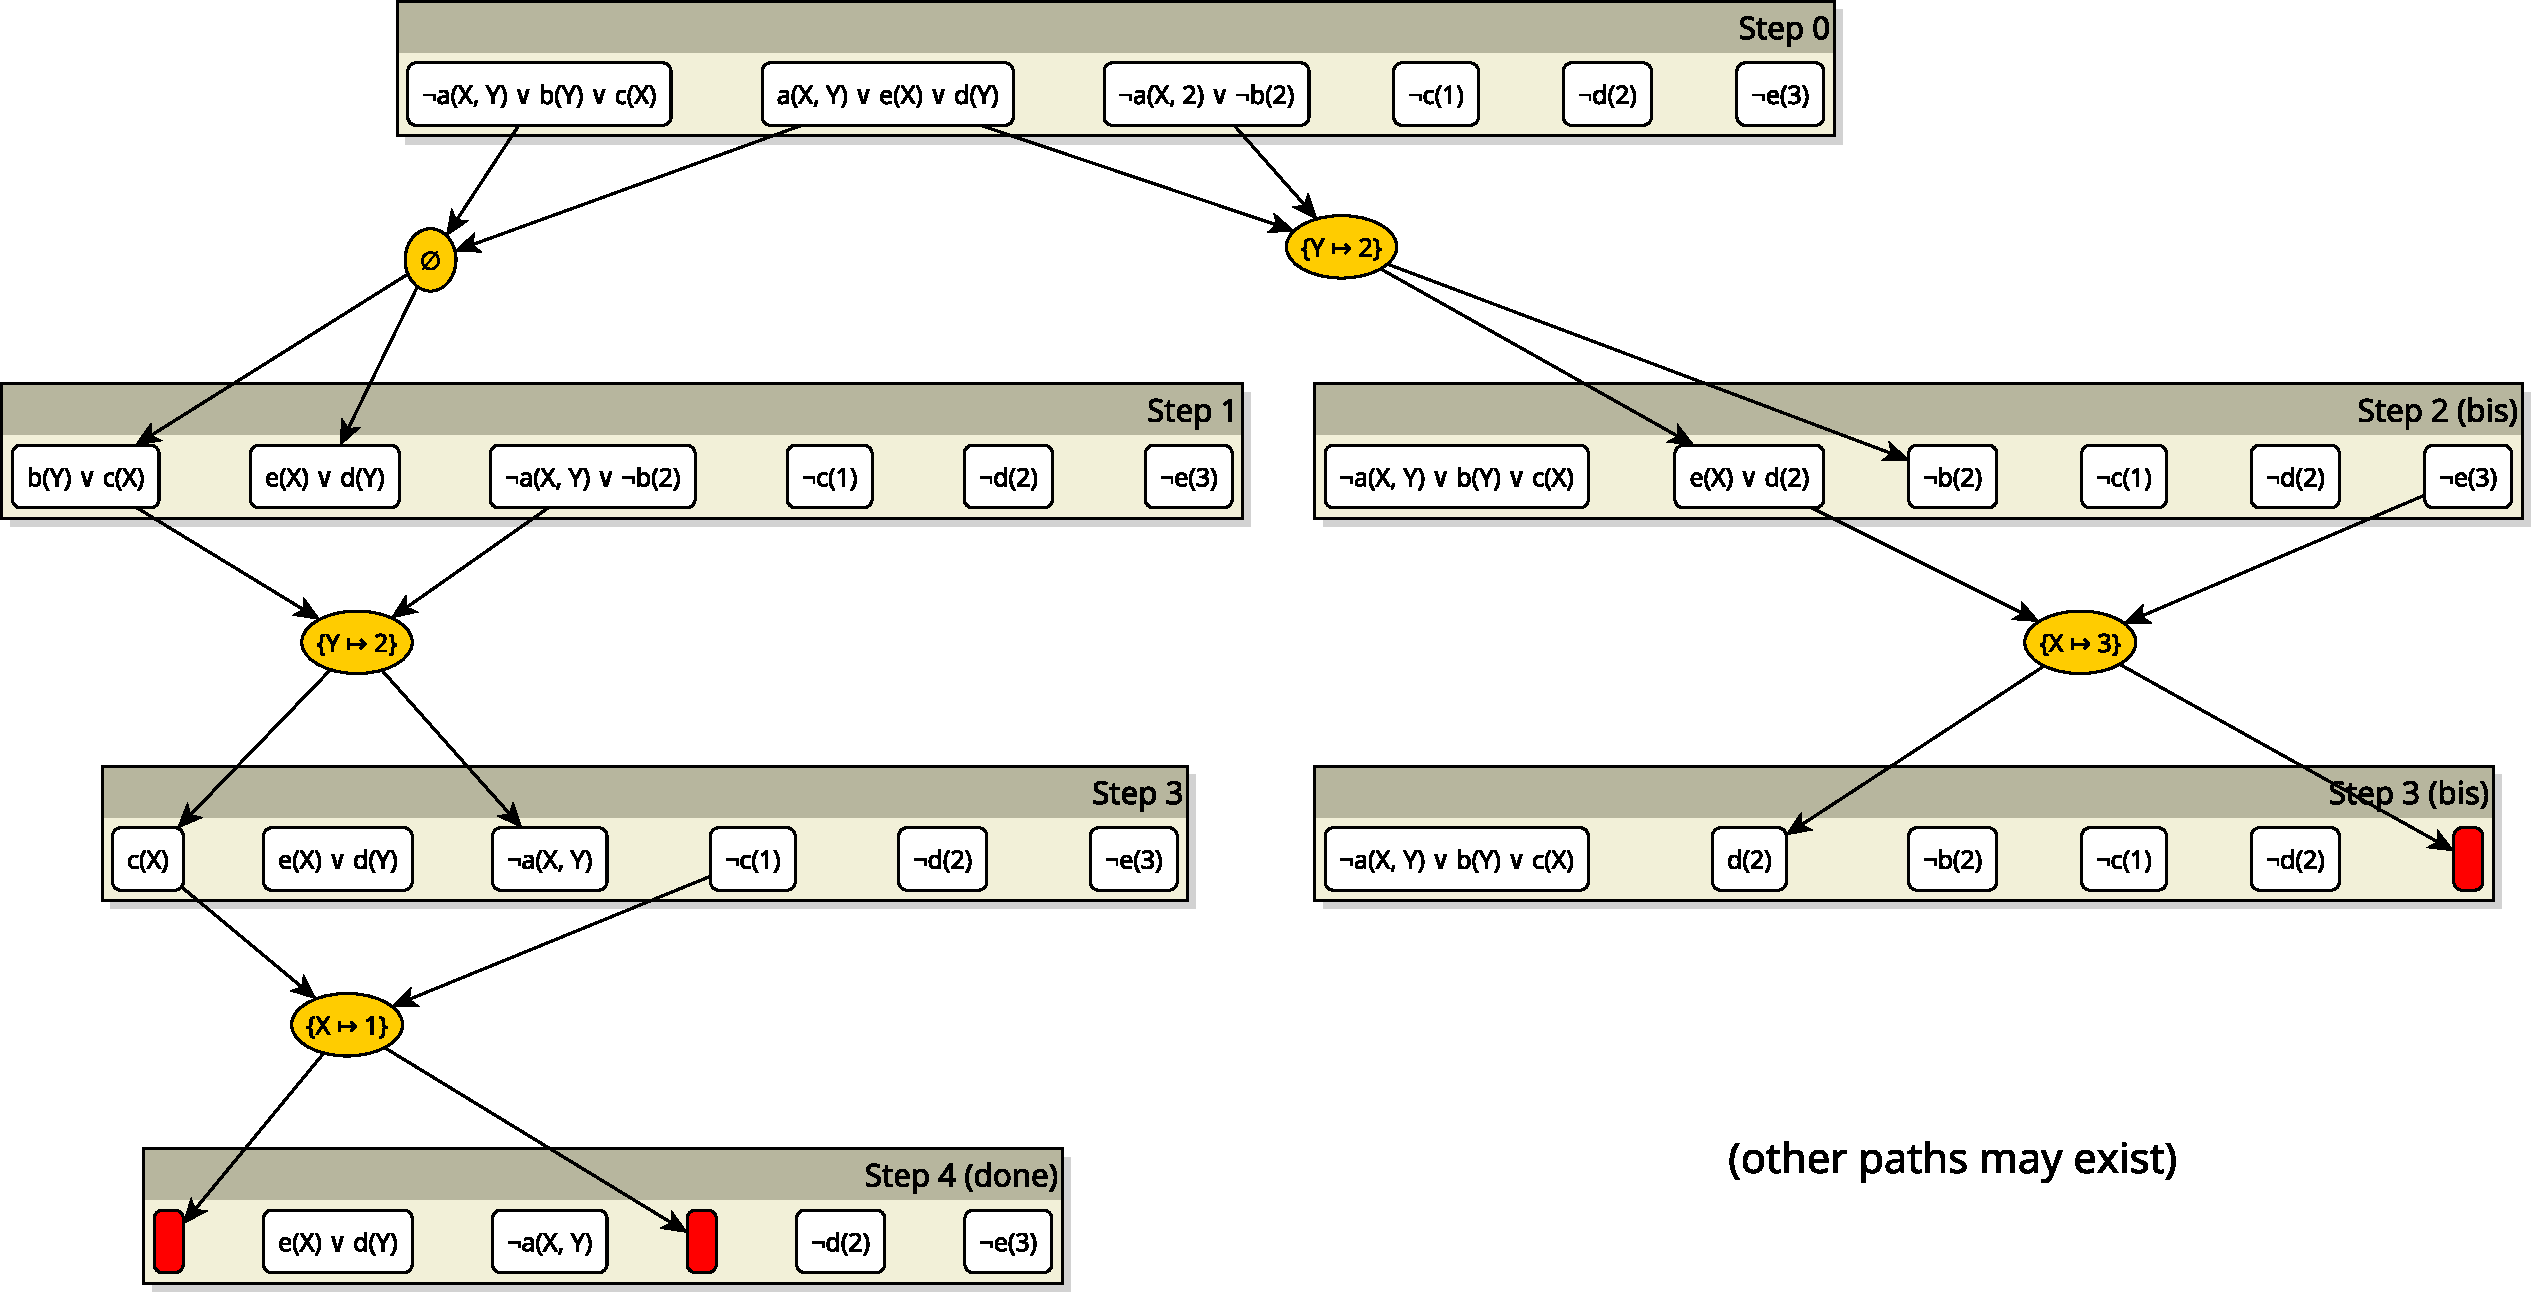
\includegraphics[width=\linewidth]{figures/sl-path-all.pdf}
    \end{figure}
\end{frame}

\begin{frame}{SL Resolution Principle -- Search Space Size}
    \begin{itemize}
        \item The proof tree is potentially \alert{huge}
        %
        \begin{itemize}
            \item exploring it all in an \alert{uninformed} way is both costly, computationally
        \end{itemize}
        
        \vfill

        \item At each step, several couples of literals may be simplified
        %
        \begin{itemize}
            \item enumerating them all is computationally expensive as well
        \end{itemize}
        
        \vfill

        \item The ordering of rewritings is \alert{relevant}
        %
        \begin{itemize}
            \item simplifications are \alert{non-commutative}
        \end{itemize}

        \vfill

        \item FOL formul\ae{} are \alert{rarely} Skolemized and in \alert{conjunctive} form
        %
        \begin{itemize}
            \item conversely, Horn clauses are Skolemized \& conjunctive \alert{by definition}
        \end{itemize}
    \end{itemize}
\end{frame}

\subsection{SLD Resolution}

\begin{frame}{SLD Resolution Principle -- Overview}
    \begin{alertblock}{SL Resolution Principle for \textbf{Definite Clauses}}
        \begin{itemize}
            \item SLD just applied SL to Horn Clauses
            
            \item Horn clauses are Skolemized \& conjunctive \alert{by definition}
            
            \item Easier to select couples of literals to be simplified
            %
            \begin{itemize}
                \item any literal in the \alert{body} of any rule \alert{unifying} with the \alert{head} of any rule
            \end{itemize}

            \item[$\rightarrow$] Procedural interpretation of resolution\ccite{KowVan1970}
            %
            \begin{itemize}
                \item[ie] literals simplification $\approx$ function call
            \end{itemize}
        \end{itemize}
    \end{alertblock}
\end{frame}

\begin{frame}[allowframebreaks]{SLD Resolution Principle -- Example}
    \begin{block}{A theory (in implication form)}
        %
        \begin{multicols}{2}
            \begin{itemize}
                \item $\predication{parent}(\functor{abraham}, \functor{isaac}) \fullstop$
                \item $\predication{parent}(\functor{isaac}, \functor{jacob}) \fullstop$
                \item $\predication{parent}(\functor{sarah}, \functor{isaac}) \fullstop$
                \item $\predication{parent}(\functor{jacob}, \functor{joseph}) \fullstop$
                \item $\predication{parent}(\functor{jacob}, \functor{dan}) \fullstop$
                \item $\predication{parent}(\functor{jacob}, \functor{dinah}) \fullstop$
                \item $\predication{male}(\functor{abraham}) \fullstop$
                \item $\predication{male}(\functor{isaac}) \fullstop$
                \item $\predication{male}(\functor{jacob}) \fullstop$
                \item $\predication{male}(\functor{joseph}) \fullstop$
                \item $\predication{male}(\functor{dan}) \fullstop$
            \end{itemize}
        \end{multicols}
        %
        \begin{itemize}
            \item $\predication{son}(X, Y) \Leftarrow \predication{parent}(Y, Y) \wedge \predication{male}(X) \fullstop$
            \item $\Leftarrow \predication{son}(S, \functor{jacob}) \fullstop$
        \end{itemize}
    \end{block}
\end{frame}

\begin{frame}[allowframebreaks]{SLD Resolution Principle -- Example}
    \begin{alertblock}{The same theory (in disjunctive form)}
        %
        \begin{multicols}{2}
            \begin{itemize}
                \item $\predication{parent}(\functor{abraham}, \functor{isaac}) \fullstop$
                \item $\predication{parent}(\functor{isaac}, \functor{jacob}) \fullstop$
                \item $\predication{parent}(\functor{sarah}, \functor{isaac}) \fullstop$
                \item $\predication{parent}(\functor{jacob}, \functor{joseph}) \fullstop$
                \item $\predication{parent}(\functor{jacob}, \functor{dan}) \fullstop$
                \item $\predication{parent}(\functor{jacob}, \functor{dinah}) \fullstop$
                \item $\predication{male}(\functor{abraham}) \fullstop$
                \item $\predication{male}(\functor{isaac}) \fullstop$
                \item $\predication{male}(\functor{jacob}) \fullstop$
                \item $\predication{male}(\functor{joseph}) \fullstop$
                \item $\predication{male}(\functor{dan}) \fullstop$
            \end{itemize}
        \end{multicols}
        %
        \begin{itemize}
            \item $\predication{son}(X, Y) \vee \neg\predication{parent}(Y, Y) \vee \neg\predication{male}(X) \fullstop$
            \item $\neg\predication{son}(S, \functor{jacob}) \fullstop$
        \end{itemize}
    \end{alertblock}

    \begin{figure}
        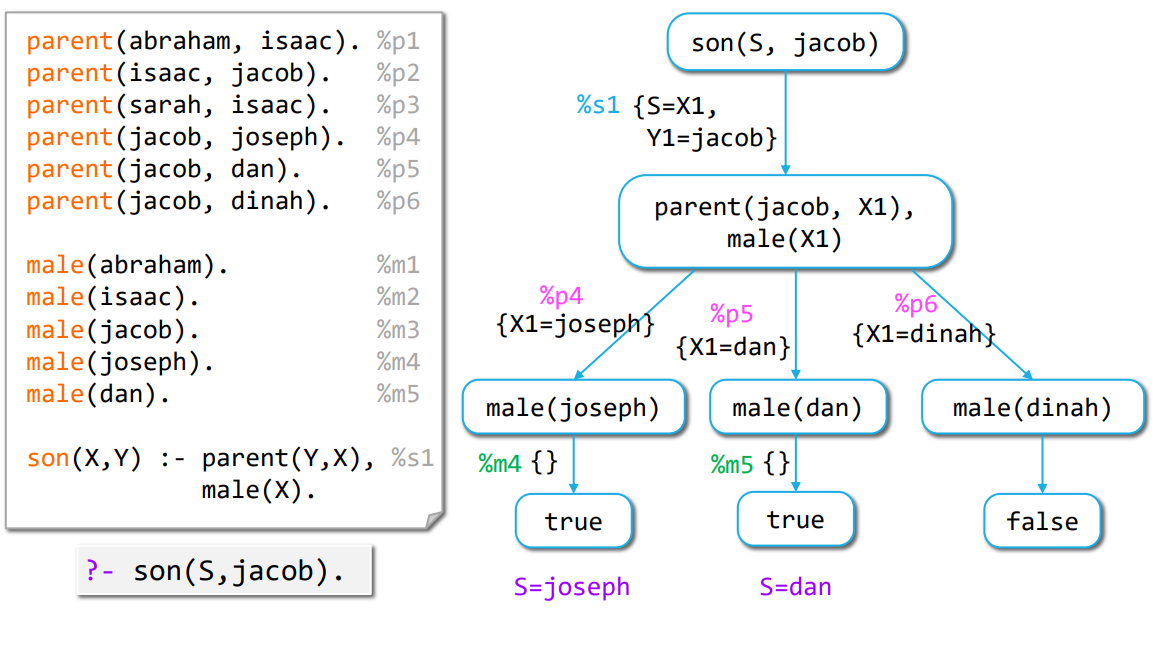
\includegraphics[width=\linewidth]{figures/proof-tree.png}
        %
        \caption{Proof tree exploration subtended by the query $\Leftarrow \predication{son}(S, \functor{jacob}) \fullstop$}
    \end{figure}
\end{frame}

\begin{frame}[allowframebreaks]{About the Proof Tree Exploration}
    \begin{itemize}
        \item SL(D) is a \alert{non-deterministic} algorithm
        %
        \begin{itemize}
            \item[ie] at any given step, several choices may be taken 
            %
            \begin{itemize}
                \item[aka] different paths may be explored
            \end{itemize} 
        \end{itemize}

        \bigskip

        \item No prescription concerning which literals should be simplified first  
        %
        \begin{itemize}
            \item[aka] which rule to try first when multiple ones could apply?
        \end{itemize}

        \bigskip

        \item Possible ways to explore the proof tree:
        %
        \begin{description}
            \item[backward chaining] (a.k.a. \emph{goal-directed}) --- start from a goal and try to solve any sub-goal implying it, recursively
            \item[forward chaining] --- start from theory and try to infer anything that can be inferred from it
        \end{description}

        \framebreak

        \item Possible search strategies to explore the proof tree:
        %
        \begin{description}
            \item[depth first] --- explore most recent goals \alert{first}
            \item[breadth first] --- explore most recent goals \alert{last} 
            \item[$\vdots$] 
        \end{description}

        \bigskip

        \item Relevant \emph{properties} a given search strategy should have: 
        %
        \begin{description}
            \item[soundness] --- \alert{any} solution found by the strategy is \alert{correct}
            \item[completeness] --- the strategy enumerates \alert{all} correct solution
        \end{description}
    \end{itemize}
\end{frame}

\begin{frame}{Proof Tree Exploration -- Example}
    \begin{figure}
        \centering
        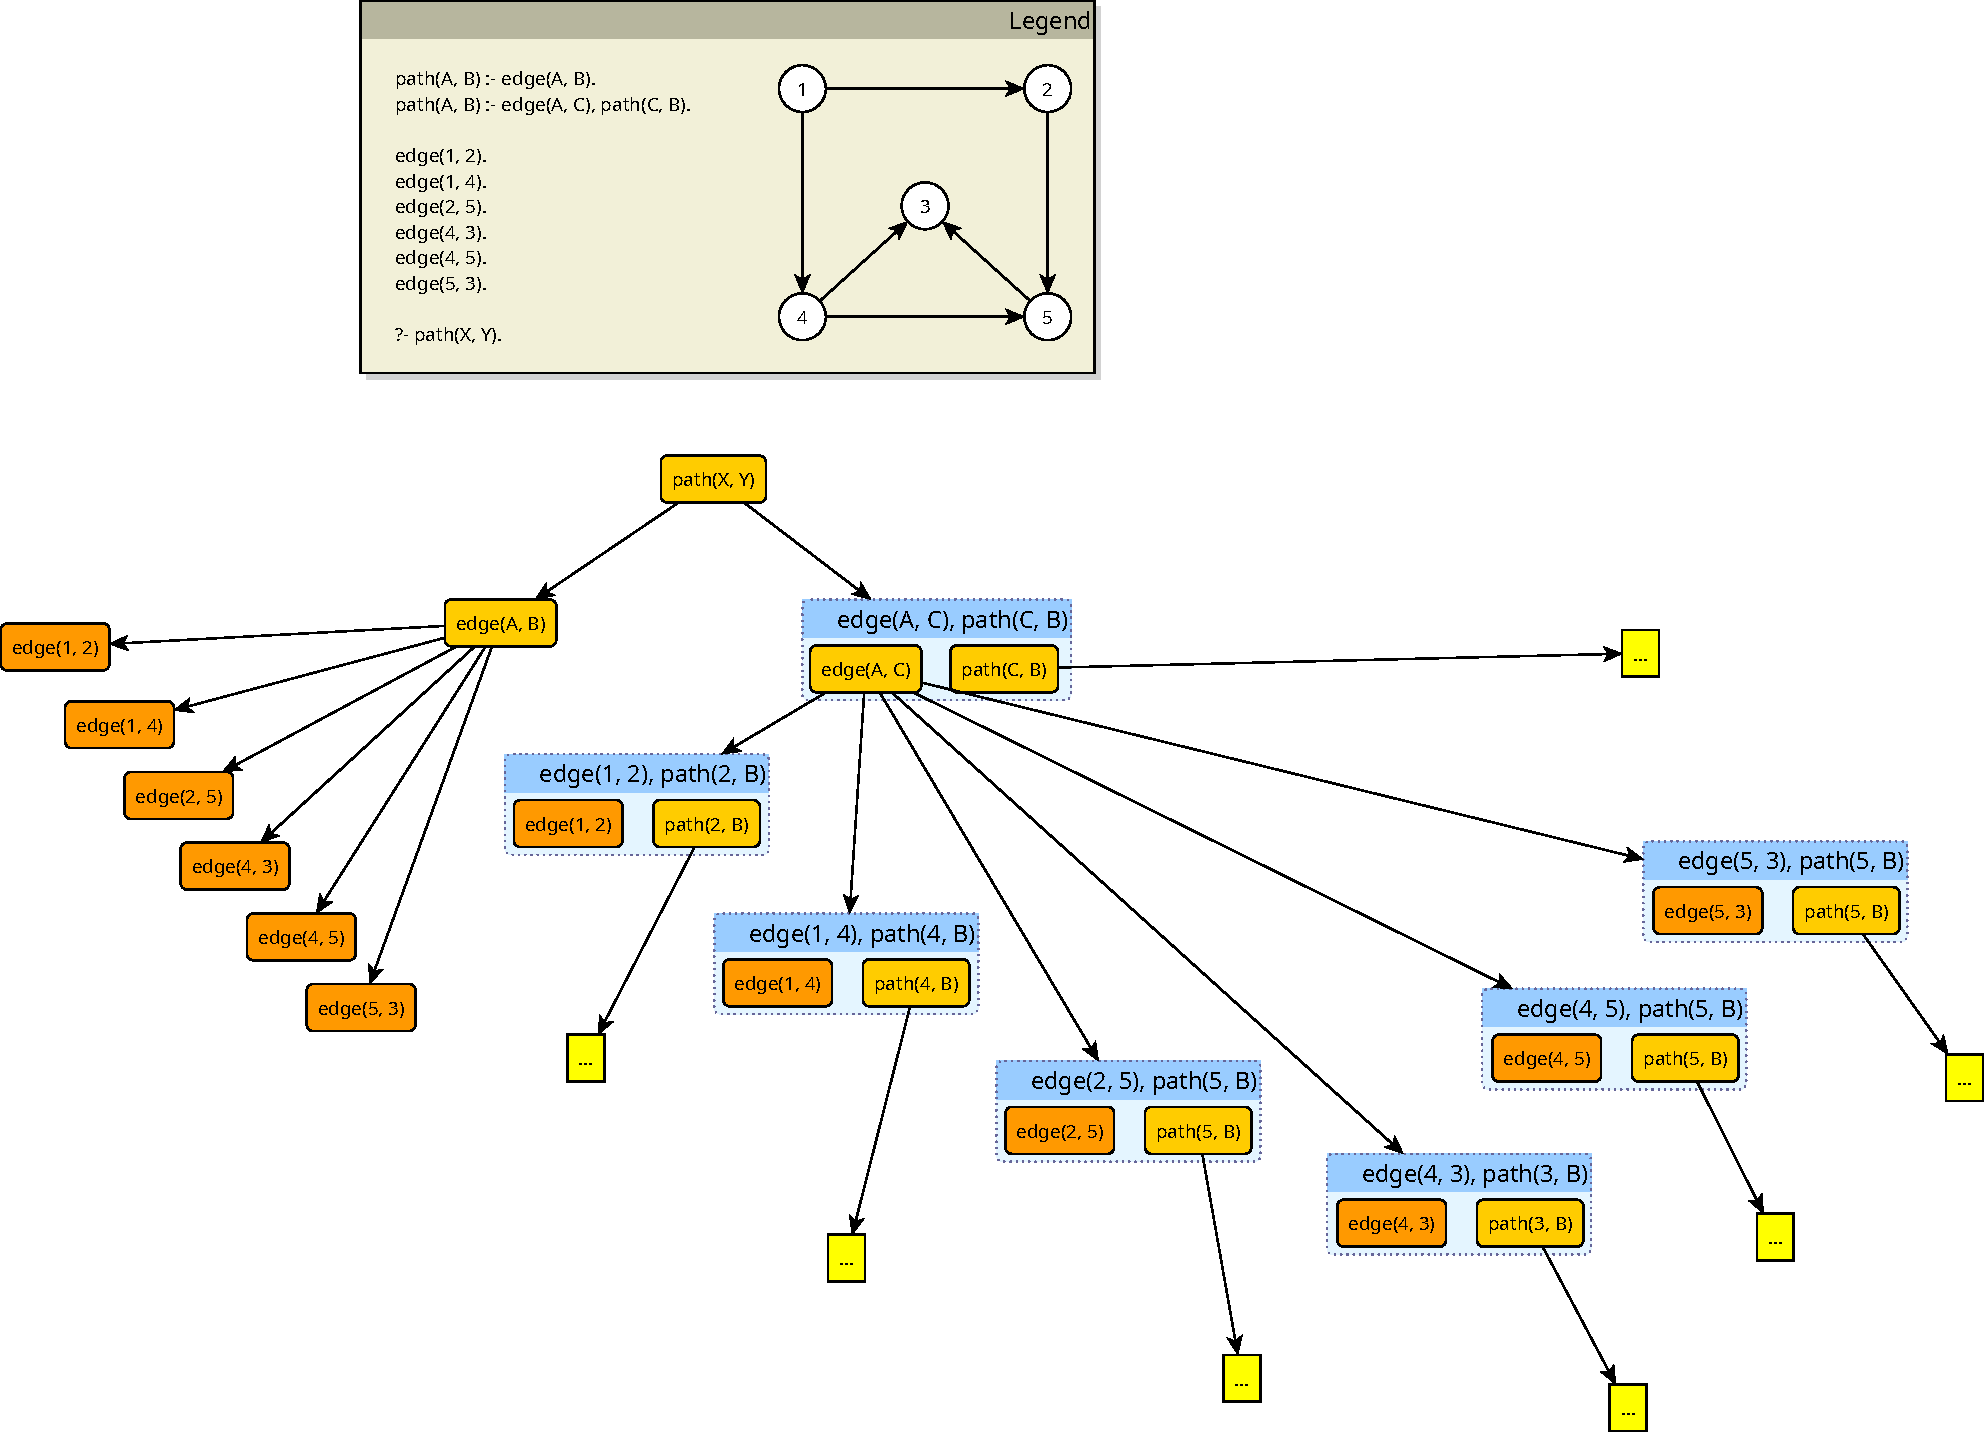
\includegraphics[width=.8\linewidth]{figures/exploration.pdf}
    \end{figure}
\end{frame}

\begin{frame}{Proof Tree Exploration -- Example (depth-first)}
    \begin{figure}
        \centering
        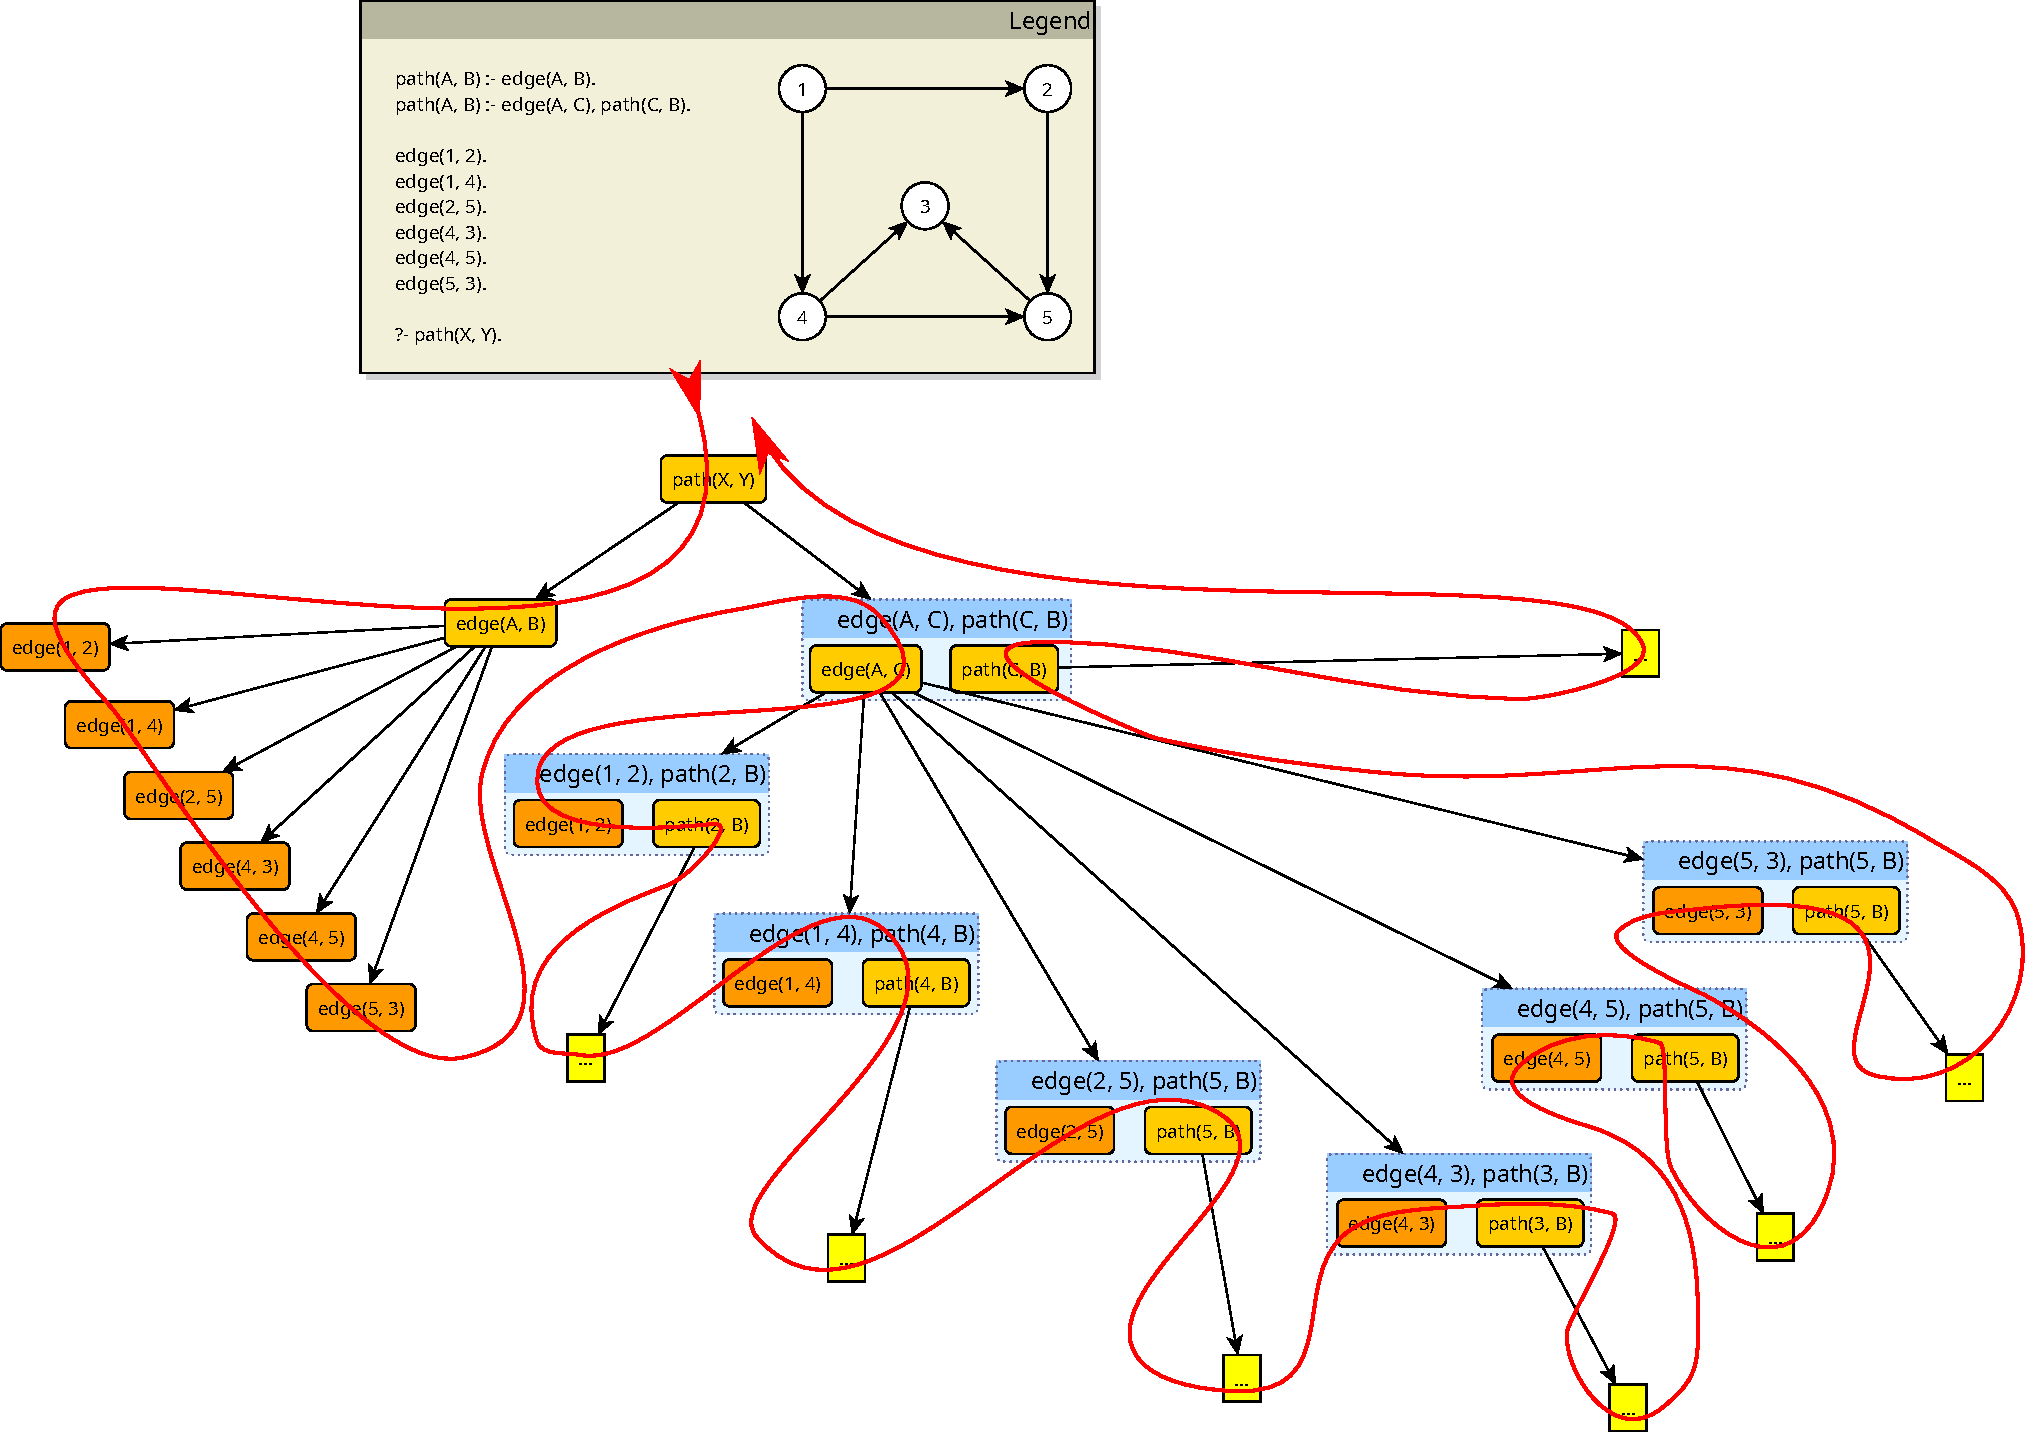
\includegraphics[width=.7\linewidth]{figures/exploration-df.pdf}
    \end{figure}
\end{frame}

\begin{frame}{Proof Tree Exploration -- Example (breadth-first)}
    \begin{figure}
        \centering
        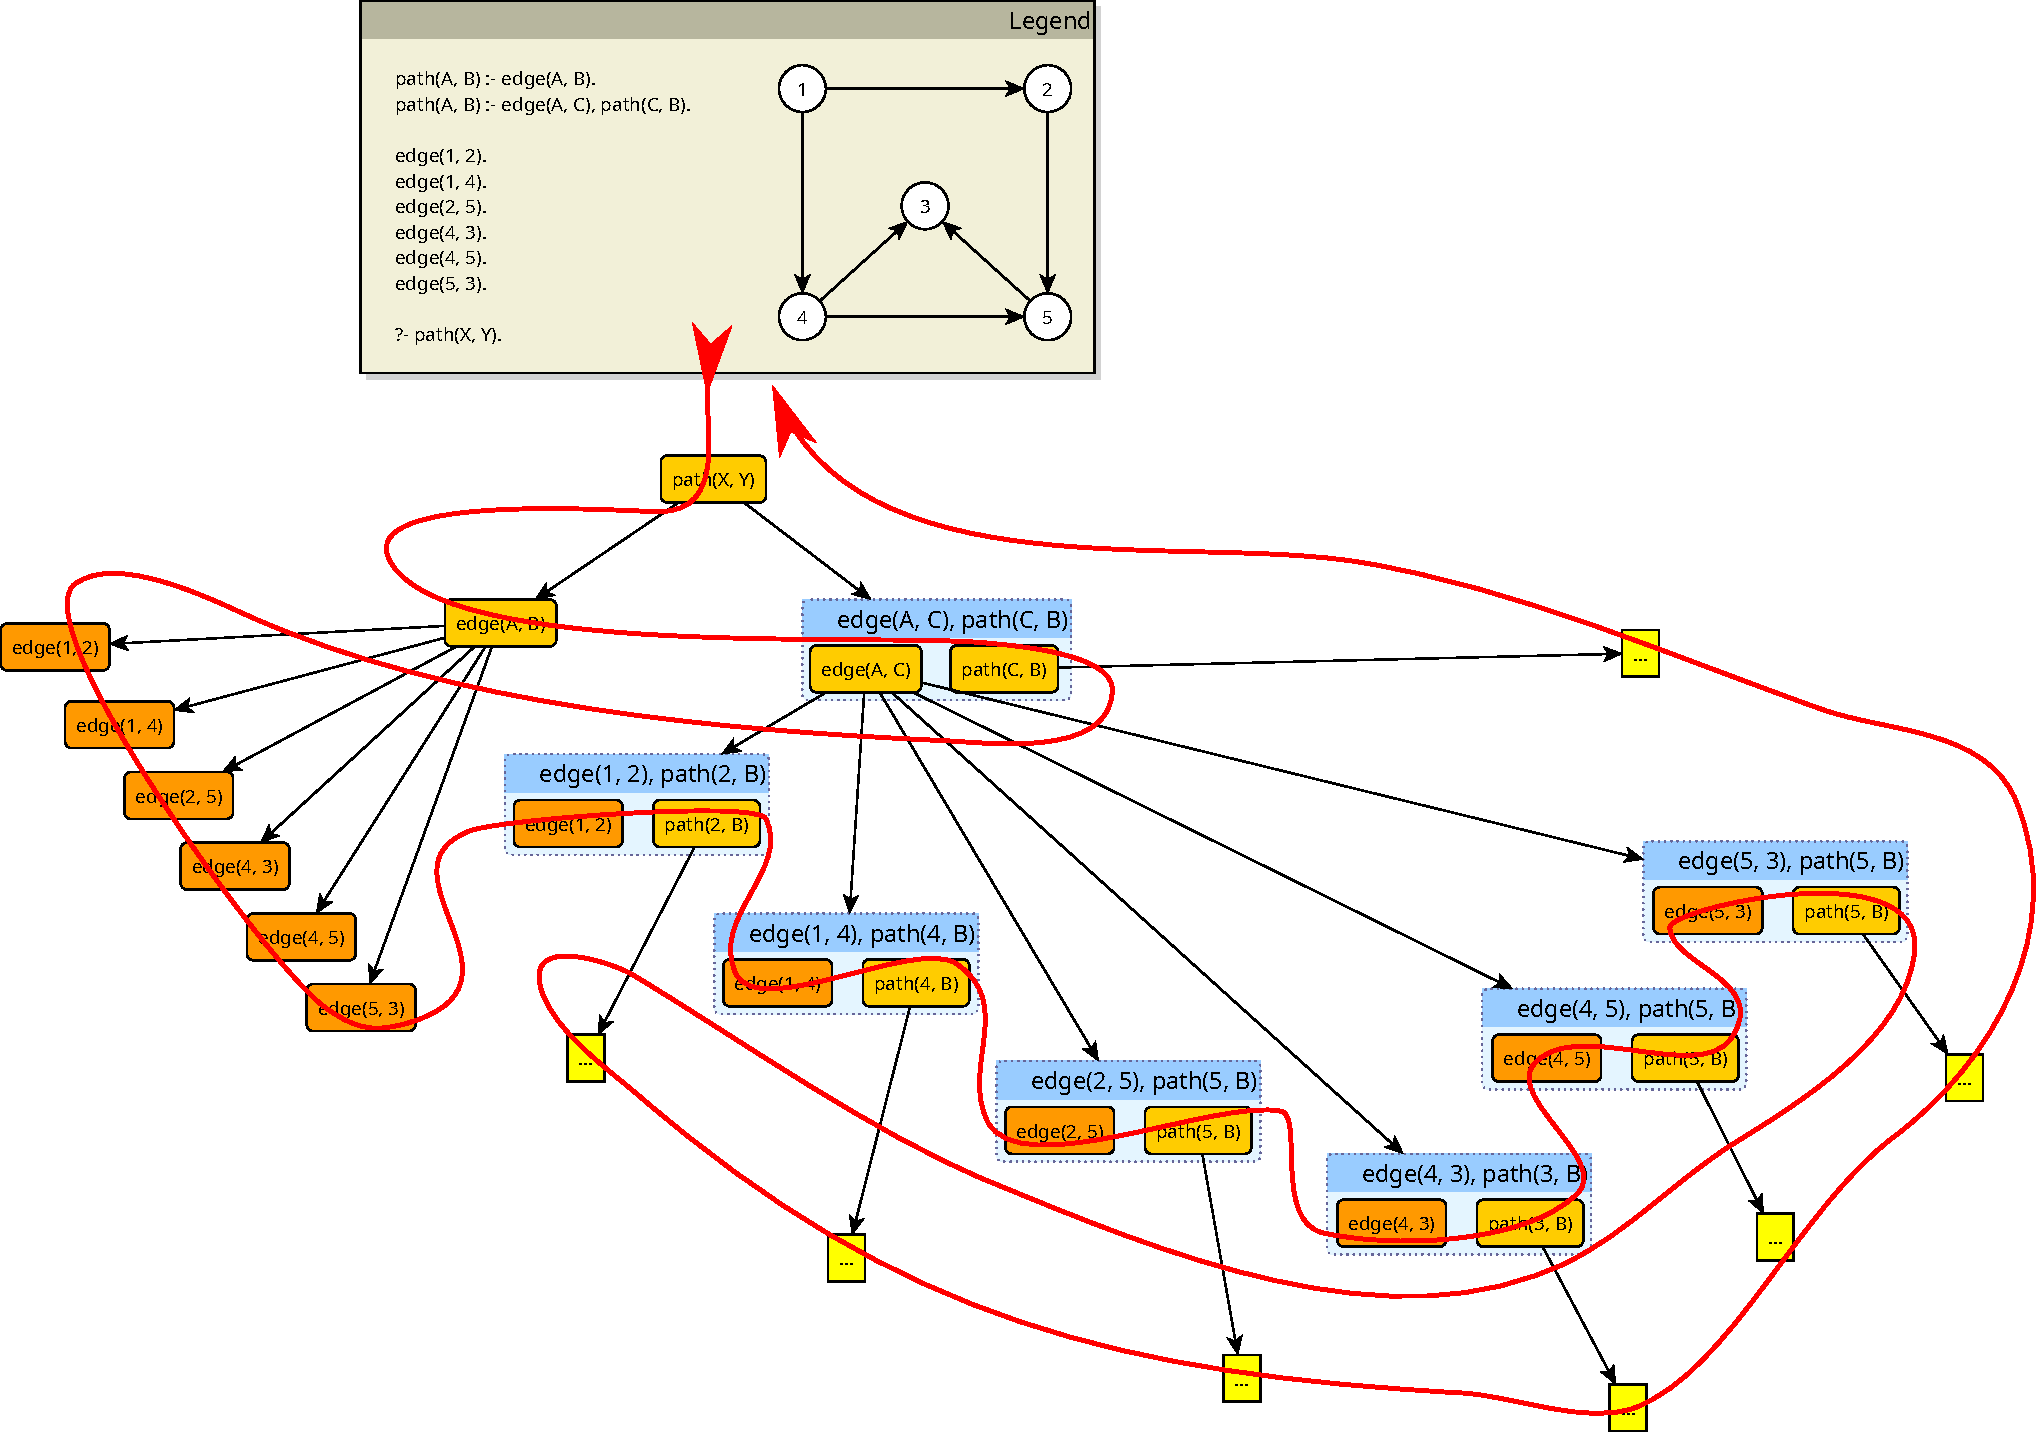
\includegraphics[width=.7\linewidth]{figures/exploration-bf.pdf}
    \end{figure}
\end{frame}

\subsubsection{Prolog}

\begin{frame}{Prolog's Proof Tree Exploration Strategy}
    \begin{itemize}
        \item Goal-directed, depth-first, sequential exploration strategy
        %
        \begin{itemize}
            \item may get stuck in recursive definitions
        \end{itemize}

        \vfill

        \item Goal-directed $\rightarrow$ \alert{procedural} interpretation of Prolog
        
        \vfill

        \item Depth-first $\approx$ \alert{left-most} goal first, \alert{top-most} rule first
        
        \vfill

        \item \alert{Backtracking} $\rightarrow$ sequential exploration
        %
        \begin{itemize}
            \item \emph{concurrent} implementations may get rid of backtracking
        \end{itemize}

        \vfill

        \item Support for \alert{side-effects} \emph{during} resolution
        %
        \begin{itemize}
            \item[eg] edits to the knowledge base (a.k.a. assertions and retractions)
            \item[eg] manipulation of exploration procedure (e.g. cut)
            \item[eg] I/O facilities via streams (a.k.a. sources and sinks) 
        \end{itemize}
    \end{itemize}
\end{frame}

%===============================================================================
\section{Exercises}
%===============================================================================

\startExercise

\begin{frame}{\currentExercise{} -- First Exercise}
	\begin{block}{Goal}
		Goal here
	\end{block}
	%
	\begin{itemize}
		\item further info here
	\end{itemize}
\end{frame}

%===============================================================================
\section*{}
%===============================================================================

%/////////
\frame{\titlepage}
%/////////

%===============================================================================
\section*{\refname}
%===============================================================================

%%%%
\setbeamertemplate{page number in head/foot}{}
%/////////
\begin{frame}[c,noframenumbering]{\refname}
%\begin{frame}[t,allowframebreaks,noframenumbering]{\refname}
%	\tiny
	\scriptsize
%	\footnotesize
	\bibliographystyle{apalike-AMS}
	\bibliography{ise-lab-inference}
\end{frame}
%/////////

%%%%%%%%%%%%%%%%%%%%%%%%%%%%%%%%%%%%%%%%%%%%%%%%%%%%%%%%%%%%%%%%%%%%%%%%%%%%%%%%
\end{document}
%%%%%%%%%%%%%%%%%%%%%%%%%%%%%%%%%%%%%%%%%%%%%%%%%%%%%%%%%%%%%%%%%%%%%%%%%%%%%%%%
